\documentclass[a0paper,portrait]{baposter}



\usepackage{wrapfig}
\usepackage{lmodern}

\usepackage[utf8]{inputenc} %unicode support
\usepackage[T1]{fontenc}


\selectcolormodel{cmyk}

\graphicspath{{figures/}} % Directory in which figures are stored


\newcommand{\compresslist}{%
\setlength{\itemsep}{0pt}%
\setlength{\parskip}{1pt}%
\setlength{\parsep}{0pt}%
}

\newenvironment{boenumerate}
  {\begin{enumerate}\renewcommand\labelenumi{\textbf\theenumi.}}
  {\end{enumerate}}



\begin{document}


\definecolor{darkgreen}{cmyk}{0.8,0.8,0,0.45}
\definecolor{lightgreen}{cmyk}{0.8,0.8,0,0.25}

\begin{poster}
{
grid=false,
headerborder=open, % Adds a border around the header of content boxes
colspacing=1em, % Column spacing
bgColorOne=white, % Background color for the gradient on the left side of the poster
bgColorTwo=white, % Background color for the gradient on the right side of the poster
borderColor=darkgreen, % Border color
headerColorOne=lightgreen, % Background color for the header in the content boxes (left side)
headerColorTwo=lightgreen, % Background color for the header in the content boxes (right side)
headerFontColor=white, % Text color for the header text in the content boxes
boxColorOne=white, % Background color of the content boxes
textborder=rounded, %rectangle, % Format of the border around content boxes, can be: none, bars, coils, triangles, rectangle, rounded, roundedsmall, roundedright or faded
eyecatcher=false, % Set to false for ignoring the left logo in the title and move the title left
headerheight=0.11\textheight, % Height of the header
headershape=rounded, % Specify the rounded corner in the content box headers, can be: rectangle, small-rounded, roundedright, roundedleft or rounded
headershade=plain,
headerfont=\Large\textsf, % Large, bold and sans serif font in the headers of content boxes
%textfont={\setlength{\parindent}{1.5em}}, % Uncomment for paragraph indentation
linewidth=2pt % Width of the border lines around content boxes
}
{}
%
%----------------------------------------------------------------------------------------
%	TITLE AND AUTHOR NAME
%----------------------------------------------------------------------------------------
%
{
\textsf %Sans Serif
{CAABOO -- Control de Arduino con Android vía Bluetooth Orientado a Objetos
}
} % Poster title
% {\vspace{1em} Marta Stepniewska, Pawel Siedlecki\\ % Author names
% {\small \vspace{0.7em} Department of Bioinformatics, Institute of Biochemistry and Biophysics, PAS, Warsaw, Pawinskiego 5a}} % Author email addresses
{\sf\vspace{0.0em}\\
Sergio Montoya y David Pachon
\vspace{0.1em}\\
\small{Departamento de Física, Universidad de los Andes, Bogotá, Colombia
\vspace{0.2em}\\
s.montoyar2@uniandes.edu.co y d.pachonb@uniandes.edu.co}
}
{
\includegraphics[scale=0.25]{logofisi.png}} % University/lab logo


\headerbox{1. Introducción}{name=introduction,column=0,row=0, span=3}{
  Arduino es una de las herramientas mas versátiles que nos ha traído la computación y la electrónica. Una de sus principales utilidades es la gran cantidad de módulos que nos permiten extender su funcionalidad. En este proyecto aprovechamos esta característica para generar un sistema de control para una habitación. Este sistema consiste en esencia de 3 módulos separados que se unen en el Arduino y son controlados por medio de una aplicación Android. El primer modulo es un sensor ultrasonido que envía una bienvenida al detectar proximidad. El segundo modulo es un micrófono que permite la transmisión de audio. El ultimo modulo es la pantalla LCD que recibe información de la aplicación y la imprime. Ademas, en el desarrollo de este proyecto no solo utilizamos herramientas útiles para el mismo si no que creamos algunas que nos permitirían desarrollar muchos mas. Como lo seria la aplicación Android.
}


\headerbox{2. Ultrasonido}{name=model,column=0,below=introduction,span=1}{
  En este caso se utilizo un modulo ultrasonido $HC-SR04$ el cual funciona enviando señal y calculando el tiempo que se demora en regresar esta señal. Con lo cual se puede calcular la distancia en función de la velocidad del sonido.
\begin{center}
    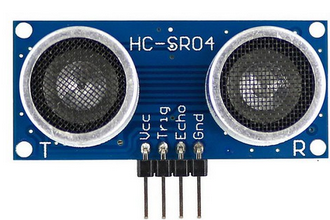
\includegraphics[width=0.8\linewidth]{ultrasonido}
\end{center}
%\vspace{-2pt}
}


\headerbox{3. Micrófono}{name=mcs,column=0,below=model,span=1}{

To measure similarity of two molecules or to combine them into one model, DeCAF first finds their \textbf{maximum common substructure (MCS)}.
To provide fast, but accurate method for solving MCS problem, we combined Generic Match Algorithm (GMA) \cite{xu1996gma} with backtracking algorithm proposed by Yiqun Cao \cite{cao2008maximum}.

Here we present comparison of molecules with similar and with different structures.
DeCAF scores and \textbf{Tanimoto coefficient (Tc)} values are shown in red and black, respectively.
\begin{center}
    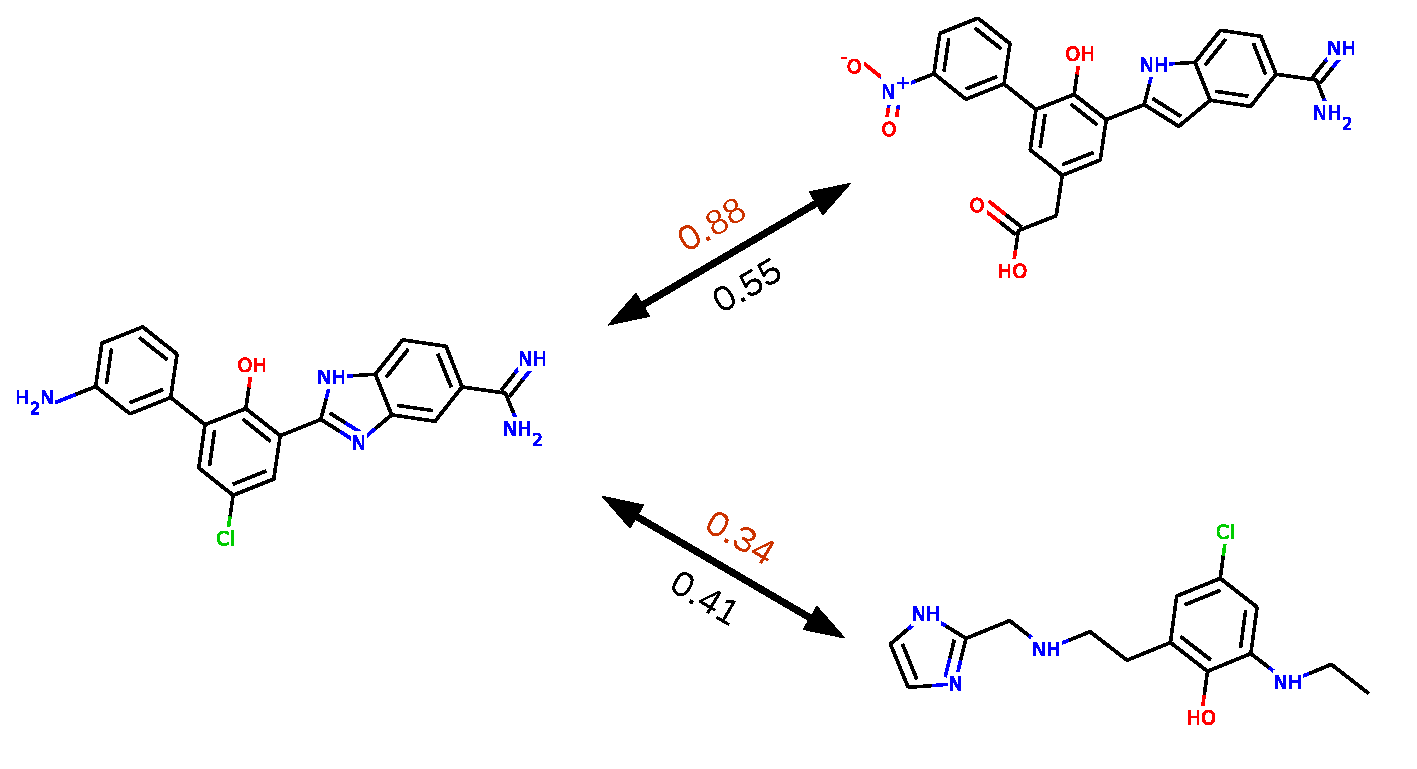
\includegraphics[width=\linewidth]{sim}
\end{center}
}

\headerbox{4. Aplicación}{name=screen,span=2,column=1,below=introduction}{
  Para la aplicación utilizamos Kotlin. En particular diseñamos un sistema de comunicación con tres botones en donde cada uno comunica por protocolo Bluetooth un carácter. Este carácter luego es recibido por el Arduino y este lo analiza. En particular hay tres vías que puede activar el carácter. La primera y segunda vía consisten simplemente en activar un output digital del Arduino. La tercera vía, por otro lado lo que hace es enviar un iniciador (Que en este caso se corresponde con el carácter $\#$) y con esto el Arduino captura un $String$ hasta que encuentra de nuevo el símbolo $\#$. 
\vspace{-5pt}
\begin{center}
    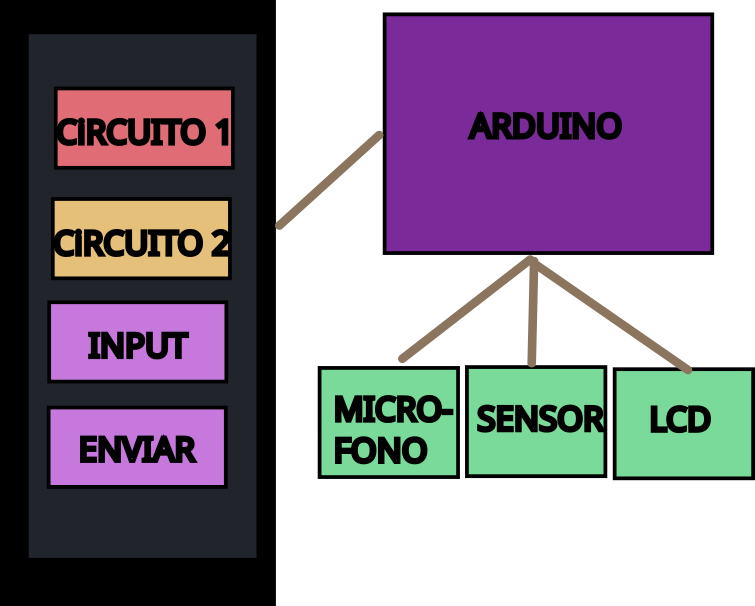
\includegraphics[width=0.45\linewidth]{esquema}
\end{center}
}


\headerbox{5. Pantalla LCD}{name=sea,span=2,column=1,below=screen}{ % To reduce this block to 1 column width, remove 'span=2'

\begin{wrapfigure}{l}{0.3\textwidth}
    \vspace{10pt}
    \begin{center}
        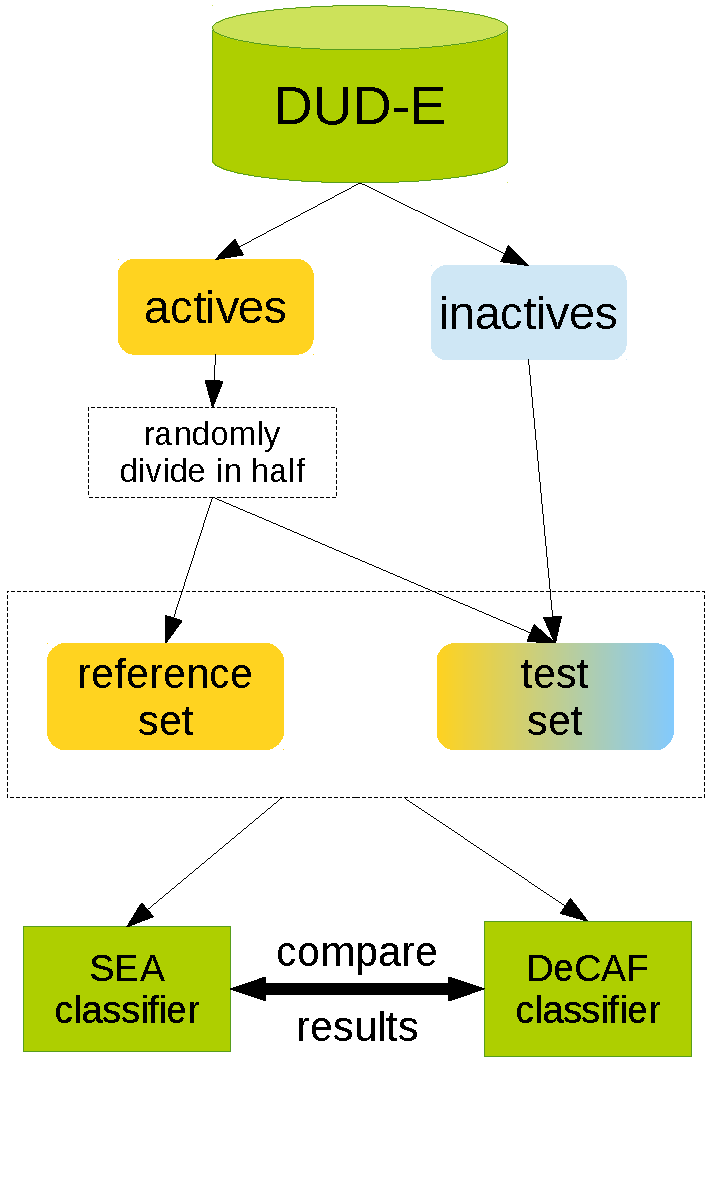
\includegraphics[width=\linewidth]{class}
    \end{center}
    %\vspace{-145pt}
\end{wrapfigure}

En este caso hicimos uso de una pantalla LCD con la cual esperabamos mostrar distintos mensajes que recibiéramos de la aplicación. Esta pantalla la acompañamos con un modulo $I^2C$ y lo programamos con la librería $LiquidCrystal\_I^2C$ con lo cual pudimos pasarle el $input$ recibido con el ultimo botón de la aplicación y mostrarlo.

\hspace{0pt}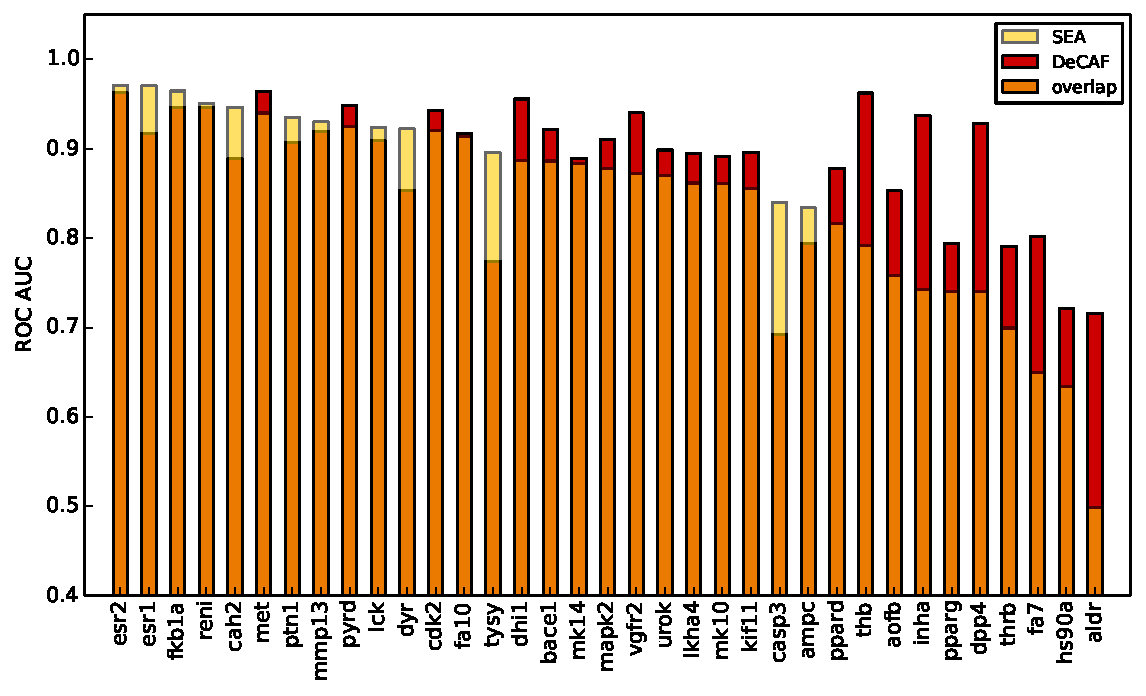
\includegraphics[width=0.95\linewidth]{res}

}


\headerbox{6. Conclusiones}{name=conclusion,column=1,below=sea,span=2,above=bottom}{
% DeCAF is a chemoinformatical tool that can be helpful in ligand-based drug design.
% It provides a comprehensive molecule description and a fast algorithms for comparing and aligning multiple ligands.
We proved that DeCAF is a significant improvement over the SEA algorithm, a popular method for comparing sets of ligands.
\begin{boenumerate}\compresslist
    \item DeCAF gives better results for 23 out of 35 receptors.
    \item For targets with easily separable active and inactive datasets, SEA and DeCAF give similar results.
    \item In cases in which SEA fails to identify active molecules, our method performs substantially better.
\end{boenumerate}
% It can be also used in other [procedures], such as database screening or drug repositioning.
% DeCAF is written in Python and freely available at \textbf{\color{darkgreen}http://bitbucket.org/marta-sd/decaf}. 
}


\headerbox{7. Referencias}{name=references,column=0,span=1,below=mcs,above=bottom}{


%\small % Reduce the font size in this block
\renewcommand{\section}[2]{\vskip 0.05em} % Get rid of the default "References" section title
%\nocite{*} % Insert publications even if they are not cited in the poster


\bibliographystyle{unsrt}
\bibliography{poster} % Use sample.bib as the bibliography file
}

\end{poster}

\end{document}
